\documentclass[11pt,a4paper]{article}
\usepackage[T1]{fontenc}
\usepackage[utf8]{inputenc}
\usepackage{lmodern}
\usepackage{amsmath,amssymb,amsthm,mathtools,mathrsfs}
\usepackage{graphicx,float,xcolor,multicol}
\usepackage[shortlabels]{enumitem}
\usepackage[margin=27mm]{geometry}
\usepackage{microtype,needspace,placeins}
\usepackage{tikz,tikz-cd}
\usetikzlibrary{arrows.meta,calc,positioning,patterns,decorations.pathreplacing}
\usepackage[colorlinks=true,linkcolor=teal,urlcolor=teal,citecolor=teal]{hyperref}
\setlength{\parindent}{0pt}
\setlength{\parskip}{.6em}
\setcounter{secnumdepth}{0}
\allowdisplaybreaks
\raggedbottom
\providecommand{\cross}{\times}
\DeclareUnicodeCharacter{2020}{\ensuremath{\dagger}}
\DeclareMathOperator{\supp}{supp}
\DeclareMathOperator*{\esssup}{ess\,sup}
\providecommand{\chapter}{\section}
\newenvironment{tool}[2]{\subsection*{Tool #1 --- #2}}{}
\newcommand{\ToolRef}[1]{Tool #1}
\newcommand{\FigureTag}[2]{\textit{Figure #1}}
\newcommand{\Result}[1]{\subsection*{#1}}
\newcommand{\Application}[1]{\subsubsection*{Application\if\relax\detokenize{#1}\relax\else\space--- #1\fi}}
\newcommand{\ProofHeading}{\par\textit{Proof.}\space}
\newcommand{\ProofOf}[1]{\par\textit{Proof of #1.}\space}
\newcommand{\RemarkHeading}{\par\textbf{Remark.}\space}
\newcommand{\NoteHeading}{\par\textbf{Note.}\space}
\newcommand{\ExerciseHeading}{\par\textbf{Exercise.}\space}

% Rendering support only; mathematical text is in each independent post.
\usepackage{booktabs,array,longtable}
\definecolor{HandoutBlue}{HTML}{2F6690}
\definecolor{HandoutNavy}{HTML}{17365D}
\newtheorem{theorem}{Theorem}
\newtheorem{lemma}[theorem]{Lemma}
\newtheorem{proposition}[theorem]{Proposition}
\newtheorem{corollary}[theorem]{Corollary}
\newtheorem{conjecture}[theorem]{Conjecture}
\newtheorem{definition}{Definition}
\newtheorem{example}{Example}
\newtheorem{namedtoolcounter}{Tool}
\newenvironment{namedtool}[1]{\begin{namedtoolcounter}[#1]}{\end{namedtoolcounter}}
\newtheorem*{claim}{Claim}
\newtheorem*{remark}{Remark}
\newtheorem*{exercise}{Exercise}
\newtheorem*{question}{Question}
\newtheorem*{observation}{Observation}
\newcommand{\SourceChapter}[2]{\section*{#2}}
\newcommand{\Lecture}[2]{\section*{Lecture #1: #2}}
\newcommand{\unclear}[1]{\textit{[unclear: #1]}}
\newcommand{\sourcegap}{\textit{[unfinished in the source]}}
\DeclareMathOperator{\dist}{dist}
\DeclareMathOperator{\id}{id}
\DeclareMathOperator{\Hol}{Hol}
\DeclareMathOperator{\Per}{Per}
\DeclareMathOperator{\Fix}{Fix}
\DeclareMathOperator{\diam}{diam}
\DeclareMathOperator{\Var}{Var}
\DeclareMathOperator{\Leb}{Leb}
\DeclareMathOperator{\Hom}{Hom}
\DeclareMathOperator{\End}{End}
\DeclareMathOperator{\Ann}{Ann}
\DeclareMathOperator{\Spec}{Spec}
\DeclareMathOperator{\Max}{Max}
\DeclareMathOperator{\Ob}{Ob}
\DeclareMathOperator{\Tor}{Tor}
\DeclareMathOperator{\Ass}{Ass}
\DeclareMathOperator{\Mor}{Mor}
\DeclareMathOperator{\Fun}{Fun}
\DeclareMathOperator{\Nat}{Nat}
\DeclareMathOperator{\Cone}{Cone}
\DeclareMathOperator{\MCG}{MCG}
\DeclareMathOperator{\Aut}{Aut}
\DeclareMathOperator{\Deck}{Deck}
\DeclareMathOperator{\SL}{SL}
\DeclareMathOperator{\PSL}{PSL}
\DeclareMathOperator{\Area}{Area}
\DeclareMathOperator{\im}{im}
\DeclareMathOperator{\PSh}{PSh}
\newcommand{\CRing}{\mathsf{CRings}}
\newcommand{\AMod}{A\text{-}\mathsf{Mod}}
\newcommand{\Ab}{\mathsf{Ab}}
\newcommand{\Z}{\mathbb Z}
\newcommand{\Q}{\mathbb Q}
\newcommand{\R}{\mathbb R}
\newcommand{\C}{\mathbb C}
\newcommand{\N}{\mathbb N}
\newcommand{\kk}{\mathbb k}
\renewcommand{\aa}{\mathfrak a}
\newcommand{\bb}{\mathfrak b}
\newcommand{\pp}{\mathfrak p}
\newcommand{\qq}{\mathfrak q}
\newcommand{\mm}{\mathfrak m}
\newcommand{\nn}{\mathfrak n}
\newcommand{\rad}{\mathrm r}
\newcommand{\cat}[1]{\mathsf{#1}}
\setcounter{secnumdepth}{0}
\allowdisplaybreaks

\graphicspath{{figures/miscellaneous/}}
\begin{document}
\section*{The Language of Category Theory (in Algebraic Topology)}
% BLOG-CONTENT-BEGIN
% Source page 1
\subsection{Philosophy in Action}
\begin{figure}[H]
 \centering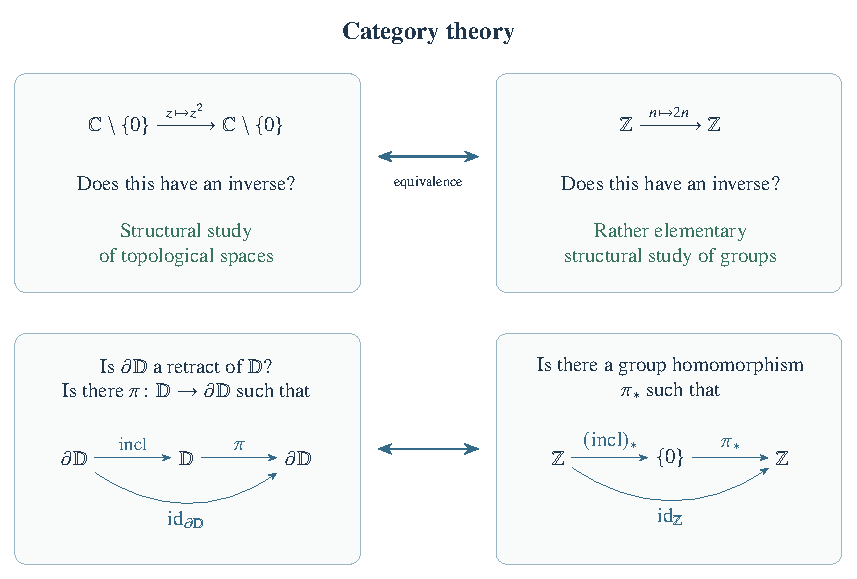
\includegraphics[width=.96\textwidth]{m1-fig-01.pdf}
 \FigureTag{M1.1}{fig:m1-fig-01}
\end{figure}

% Source page 2
\setcounter{example}{0}\begin{example}
$\cat{Sets}$, $\cat{Grps}$, $\cat{Rings}$, $\cat{Top}$,
$k\text{-}\cat{Top}$, $\cat{Top}_*$, $k\text{-}\cat{Top}_*$,
$k\text{-}\cat{Top}_*/{\sim}$, $\cat{CRings}$, $\cat{Man}$, $\ldots$.
\end{example}
\setcounter{definition}{1}\begin{definition}[Functor]
For categories $\mathcal C$ and $\mathcal D$, a functor
$F\colon\mathcal C\to\mathcal D$ gives maps
$F\colon\Ob(\mathcal C)\to\Ob(\mathcal D)$ and
$F\colon\Mor(\mathcal C)\to\Mor(\mathcal D)$ such that
\[
 F(*\xrightarrow{f}*)=\bigl(F(*)\xrightarrow{F(f)}F(*)\bigr),\qquad
 F(\id_*)=\id_{F(*)},\qquad F(f\circ g)=F(f)\circ F(g).
\]
\end{definition}
Functors give us ways to understand certain relations in a category better
by translating them to a different category. Given two such translations,
is there a way not to get lost in translation?
\setcounter{definition}{2}\begin{definition}[Natural transformation]
Let $F,G\colon\mathcal C\to\mathcal D$ be two functors. A natural
transformation is a collection of morphisms
$\{\nu_A\}_{A\in\Ob(\mathcal C)}$ such that the following square commutes.
\begin{figure}[H]
 \centering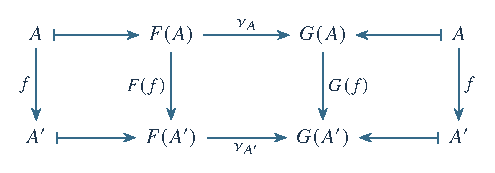
\includegraphics[width=.78\textwidth]{m1-fig-03.pdf}
 \FigureTag{M1.3}{fig:m1-fig-03}
\end{figure}
We say that $\{\nu_A\}_{A\in\Ob(\mathcal C)}$ is a \emph{natural isomorphism}
if $\nu_A$ is an isomorphism for every $A\in\Ob(\mathcal C)$.
\end{definition}

% Source page 3
\paragraph{Principle.}
Every statement in category theory has a dual statement obtained by replacing
$f\circ g$ with $g\circ f$ and domain with codomain, essentially flipping the
arrows of the morphisms.

Let us now look at some examples to gather some context. But before that,
a small digression. In set theory, certain sets, such as the set of all
groups or the set of all singletons, cannot exist. Hence the need to write
a new set of axioms to create what are called classes, whose elements are
sets that satisfy given properties. But for our purposes, let us stick to
small or locally small categories, thereby avoiding the set-versus-class
conundrum.
\subsection{Some Pillars of Category Theory}
\subsubsection{Functor Categories}
Let $\mathcal C=\Fun(\mathcal A,\mathcal B)$, where $\mathcal A$ and
$\mathcal B$ are categories. Its objects are functors
$F\colon\mathcal A\to\mathcal B$, and its morphisms are natural transformations.
We say $\mathcal C\cong\mathcal D$ if there exist
$F\colon\mathcal C\to\mathcal D$ and $G\colon\mathcal D\to\mathcal C$ such that
$F\circ G=\id_{\mathcal D}$ and $G\circ F=\id_{\mathcal C}$.
We say $\mathcal C\sim\mathcal D$ if
$F\circ G\sim\id_{\mathcal D}$ and $G\circ F\sim\id_{\mathcal C}$,
via natural isomorphisms.
\subsubsection{Representable Functors}
For $X,C\in\Ob(\mathcal C)$, define
$h_X\colon\mathcal C^{\mathrm{op}}\to\cat{Sets}$ by
% Source page 4 (the defining formula overlaps the previous page boundary).
\[
 h_X(C)=\Hom(C,X),\qquad
\]
We say that a functor $F\colon\mathcal C^{\mathrm{op}}\to\cat{Sets}$ is
\emph{representable} if there exists $C\in\Ob(\mathcal C)$ such that $F\cong h_C$.

Everything in category theory can be studied via appropriate representable
functors. This is akin to studying the category $\mathcal C$ by acting it on
$\mathcal C$, where the action is given by $\Hom_{\mathcal C}(-,-)$.
\subsubsection{Adjunctions (or Adjoints)}
Let $\mathcal C$ and $\mathcal D$ be two categories, and let
$F\colon\mathcal C\to\mathcal D$ be a functor. An adjoint to $F$ is a
functor $G\colon\mathcal D\to\mathcal C$ such that
\[
 \Hom_{\mathcal C}(C,G(D))\cong\Hom_{\mathcal D}(F(C),D).
\]
\subsection{Constructing New Categories from Old}
\subsubsection{Subcategory}
The definition is obvious.
\subsubsection{Comma Category}
Let $\mathcal C$ be a given category and $B\in\Ob(\mathcal C)$.
Write $\mathcal C\downarrow B$ for the \emph{comma category over $B$}.
Its objects are maps in $\mathcal C$, of the form $X\xrightarrow{\pi}B$
(a ``$B$-parametrized family of objects in $\mathcal C$'').
The set
\[
 \Hom_{\mathcal C\downarrow B}
 \bigl((X\xrightarrow{\pi}B),(X'\xrightarrow{\pi'}B)\bigr)
\]
consists of the maps $f\colon X\to X'$ for which the following diagram commutes.
\begin{figure}[H]
 \centering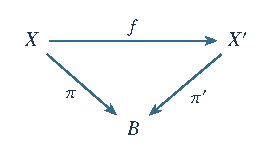
\includegraphics[width=.30\textwidth]{m1-fig-07.pdf}
 \FigureTag{M1.7}{fig:m1-fig-07}
\end{figure}
The dual notion is $B\downarrow\mathcal C$.
\setcounter{example}{3}\begin{example}
If $\mathcal C=\cat{Top}$ and $B=\{*\}$, then
$B\downarrow\mathcal C=\cat{Top}_*$ (based spaces).
\end{example}
Finally, $A\downarrow\mathcal C\downarrow B:=A\downarrow(\mathcal C\downarrow B)$
demands that the following diagram commute.
% Source page 11
\begin{figure}[H]
 \centering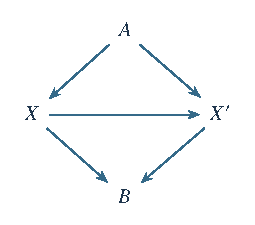
\includegraphics[width=.28\textwidth]{m1-fig-08.pdf}
 \FigureTag{M1.8}{fig:m1-fig-08}
\end{figure}
\subsubsection{Category of Presheaves}
Given a category $\mathcal C$, define $\PSh(\mathcal C)$ by taking functors
$F\colon\mathcal C^{\mathrm{op}}\to\cat{Sets}$ as objects and natural
transformations as morphisms. Thus
$\PSh(\mathcal C)=\Fun(\mathcal C^{\mathrm{op}},\cat{Sets})$.
\subsection{Standard Instances}
\subsubsection{Objects as Morphisms}
Let $X\in\Ob(\mathcal C)$. The points of $X$ can be thought
% Source page 12
of as $\Hom_{\mathcal C}(*,X)$, where $*$ is a final object in $\mathcal C$.
``Generalized points'' can be thought of as $\Hom_{\mathcal C}(A,X)$.
We are simply generalizing these notions from $\mathcal C=\cat{Sets}$,
where $*$ is a singleton set, and morphisms from $*$ to $X$ in $\cat{Sets}$
give a correspondence with points of $X$.
\subsubsection{Groups as Categories}
Given a group $G$, define a category $\mathcal BG$ as follows:
\[
 \Ob(\mathcal BG):=\{*\}\quad\text{(a singleton)},\qquad
 \Mor(\mathcal BG):=G,
\]
where $g\in G$ is a morphism $*\to*$ and multiplication is composition.
\subsubsection{Forgetful Functors}
Let $\mathcal C$ be a category of certain sets with a particular
% Source page 13
structure imposed. The forgetful functor is
\[
 U\colon\mathcal C\to\cat{Sets},\qquad
 U(C)=C\quad\text{(the underlying set)},\qquad
 U(f\colon C\to D)=f\colon C\to D\quad\text{(the set map)}.
\]
\subsection{Certain Limit Constructions in Algebraic Topology}
\subsubsection{Products and Coproducts}
Let $\{X_i\}_{i\in I}$ be objects in $\mathcal C$. Consider the discrete
category $X$, with $\Ob(X)=X_i$ and $\Mor(X)=\id_{X_i}$, and let
$\chi\colon X\hookrightarrow\mathcal C$ be the inclusion.
The limit and colimit of $\chi$, if they exist, are products and coproducts.
In $\cat{Top}$, the product is $\prod_{i\in I}X_i$, with the product topology,
and the coproduct is $\coprod_{i\in I}X_i$.
In $*\downarrow\cat{Top}\sim\cat{Top}_*$, the product of the $(X_i,x_i)$ is
$\bigl(\prod_{i\in I}X_i,\{x_i\}_{i\in I}\bigr)$ and the coproduct is
$\bigvee_{i\in I}(X_i,x_i)$.
\begin{remark}
The limit and colimit of a diagram are essentially two ways of putting
objects together such that the relations between them are preserved.
\end{remark}
In $\cat{Top}$, putting together $A\xrightarrow{f}X$ and $A\xrightarrow{g}Y$
would give $(X\amalg Y)/\{f(x)\sim g(x):x\in A\}$.
In $\cat{Grps}$, putting together the same diagram would give
\[
 (X*Y)/N\bigl(f(a)g(a)^{-1}:a\in A\bigr),
\]
the amalgamated product.
Essentially, given $\mathcal C$, one has to look for appropriate analogues
of $\prod$ and $\coprod$, and then put objects together preserving the
relations in the diagram.

Having seen all this, let us (sort of) look at the only lemma in category theory.
\setcounter{theorem}{0}\begin{lemma}[Yoneda's lemma]\label{lem:m1-yoneda}
Let $F\in\PSh(\mathcal C)$. For any $X\in\Ob(\mathcal C)$, there is an
isomorphism of sets
\[
 \Hom_{\PSh(\mathcal C)}(h_X,F)\cong F(X)
\]
that is natural in both $X$ and $F$.
\end{lemma}
% Source page 18: blank.
% Source page 19
\begin{proof}[Sketch of proof]
Suppose $\theta\in\Hom_{\PSh(\mathcal C)}(h_X,F)$, i.e.
$\{\theta_A\colon h_X(A)\to F(A)\}_{A\in\Ob(\mathcal C)}$.
Define
\[
 \Phi\colon\Hom_{\PSh(\mathcal C)}(h_X,F)\to F(X),\qquad
 \Phi\bigl(\{\theta_A\}_{A\in\Ob(\mathcal C)}\bigr)=\theta_X(\id_X).
\]
Let $a\in F(X)$. Then $\Psi(a)\in\Hom_{\PSh(\mathcal C)}(h_X,F)$ is given by
\[
 \Psi(a)_A(f):=F(f)(a)\qquad(f\in h_X(A)),
\]
the natural evaluation. Verify the rest.
\end{proof}
Let $\mathcal C$ be a category and $X\in\Ob(\mathcal C)$. Then
$X$ is a group object if and only if $h_X\colon\mathcal C^{\mathrm{op}}\to\cat{Sets}$
lifts to groups, i.e. there exists $\widetilde h_X$ making the following
diagram commute; $U$ is the forgetful functor.
\begin{figure}[H]
 \centering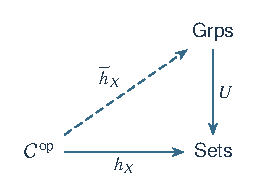
\includegraphics[width=.43\textwidth]{m1-fig-15.pdf}
 \FigureTag{M1.15}{fig:m1-fig-15}
\end{figure}
% BLOG-CONTENT-END
\end{document}
